% 2026-10-26 (integration, JFEc): Section 6 (Results) holds two floats, Table 1 (tab:rh_oos) and the ablation table
% (tab:rh_ablation). The calibration table and figure of the MSE/QLIKE discussion (tab:rh_calibration,
% fig:rh_calibration) are in rehaul/A_results.tex; the MCS tables (tab:rh_mcs, tab:rh_mcs_spa) and the closing-bar
% table (tab:rh_close_accuracy) are the APPENDIX agent's. Everything parked below stays parked.
% 06_results_floats.tex -- tables and figures for this section (2026-10-15), each \input from a generated/ file or an
% \includegraphics of a generated figure; generators: writeup/make_rehaul_*.py. Placed after the section in paper_rehaul.tex
% so section text and floats can be edited in parallel; move them inline when the prose settles.
%
% Generator: writeup/make_rehaul_results.py (tables generated/rehaul_results_t*.tex, figures
% figures/rehaul_results_f*.pdf, caption numbers generated/rehaul_results_numbers.tex as \rhr... macros). It asserts the
% outline's numbers (writeup/PAPER_REHAUL_OUTLINE_2026-10-15.md, section 6) before writing anything.
% Conventions everywhere (2026-10-15 consolidation): variance forecast \hat\sigma^2_t = \hat y_t^2 s^2_{t,c}, scored
% against the actual RV over the \rhrDays trading days of the out-of-sample period; DM = dm_test (Bartlett Newey-West,
% q_NW = \rhrDMLag, HLN correction, normal p); the Sharpe-ratio change is tested by newey_west_t (q_NW = \rhrHACLag);
% stars for the 10/5/1 % levels. Model-class colors and markers (= make_rehaul_economics.py): closing-interval linear
% blue circle, trees vermilion square, MinGRU green triangle, pooled intraday magenta diamond. The full ranking
% (tab:rh_rank_full) is in the appendix; the estimation-sample sign convention is pooled minus closing-interval.
% Labels: tab:rh_axis1 (T1), tab:rh_axis2 (T2), tab:rh_rank (T3), tab:rh_rank_full (T3, every forecast);
% fig:rh_axis1_forest (F1), fig:rh_pooled_dumbbell (F2), fig:rh_cumulative (F3), fig:rh_se_share (F5),
% fig:rh_qlike_sharpe (the existing QLIKE-vs-Sharpe figure).
% The pooled ridge-init MinGRU (results/puffer_forecast_2026-10-12/pooled_rinit_study/, refit monthly) is in T1, T2,
% T3, F1 and F2 since 2026-10-15; the pooled forest on all features is still interim (dagger).
% 2026-10-15 (finish, user): NN content parked -- the MinGRU leaves fig:rh_cumulative's caption (the generator agent
% removes it from T1-T3 and the figure).

% 2026-10-15 (consolidation): parked -- the number files are loaded once in the preamble of paper_rehaul.tex (the first
% line was an unguarded second load of rehaul_results_numbers).
% % AUTO-GENERATED by writeup/make_rehaul_results.py -- do not edit.
% Numbers for the captions of writeup/rehaul/06_results_floats.tex (plain f^2 B, 866 days, DM lag 6 HLN).
\providecommand{\rhrDays}{866}  % trade days scored
\providecommand{\rhrNNPooledSeeds}{3}  % seeds averaged in the pooled MinGRU forecast
\providecommand{\rhrOlsQ}{0.0946}  % QLIKE of the per-bar OLS on HAR + calendar
\providecommand{\rhrAfPairs}{51}  % model-set input-set pairs (all features vs HAR + cal.)
\providecommand{\rhrAfLower}{38}  % ... QLIKE lower with all features
\providecommand{\rhrAfLowerSig}{2}  % ... and DM p < 0.05
\providecommand{\rhrAfMseHigher}{51}  % ... variance-space MSE higher with all features
\providecommand{\rhrAfMseHigherSig}{0}  % ... and DM (squared error) p < 0.05
\providecommand{\rhrNModelSet}{112}  % forecasts in the master table's model set
\providecommand{\rhrRankN}{120}  % forecasts ranked in the full table
\providecommand{\rhrNSet}{111}  % model-set forecasts other than the OLS
\providecommand{\rhrNLower}{7}  % ... with lower QLIKE than the OLS
\providecommand{\rhrNLowerSig}{0}  % ... and DM p < 0.05
\providecommand{\rhrNWorseSig}{48}  % ... significantly worse than the OLS (DM p < 0.05)
\providecommand{\rhrLinBaseMaxPct}{0.03}  % largest |% change| of the per-bar ridge / lasso / enet on HAR + cal. vs the OLS
\providecommand{\rhrSETopFiveOls}{88}  % % of the OLS's total squared error on its 5 largest days
\providecommand{\rhrSETopFiveMin}{85}  % min over the four F5 forecasts: % of squared error on the 5 largest days
\providecommand{\rhrSETopFiveMax}{92}  % max over the four F5 forecasts
\providecommand{\rhrQLTopFiveMin}{7}  % min over the four F5 forecasts: % of total QLIKE on the 5 largest days
\providecommand{\rhrQLTopFiveMax}{9}  % max over the four F5 forecasts
\providecommand{\rhrCumLassoTotal}{\ensuremath{-}2.76}  % lasso, all features: sum over days of the QLIKE difference vs the OLS
\providecommand{\rhrCumLassoWindow}{\ensuremath{+}1.60}  % ... of which in 24 Feb - 30 Apr 2020
\providecommand{\rhrCumXgbTotal}{\ensuremath{-}0.98}  % XGBoost (daily refit), all features: sum over days
\providecommand{\rhrCumXgbWindow}{\ensuremath{+}0.30}  % ... of which in 24 Feb - 30 Apr 2020
\providecommand{\rhrCumNnTotal}{\ensuremath{+}0.16}  % MinGRU, all features: sum over days
\providecommand{\rhrCumNnWindow}{\ensuremath{+}0.78}  % ... of which in 24 Feb - 30 Apr 2020

% \ifdefined\fqsPairs\else% AUTO-GENERATED by writeup/make_fig_qlike_sharpe.py -- do not edit.
% Figure writeup/figures/fig_qlike_sharpe.pdf: QLIKE against Sharpe (mid), HAR + calendar vs all
% features, every model of results/close_master_table/paper_model_set.csv on both input sets
% (per-bar linear = the pre-tuned subpt_* rows; LSTMs excluded); numbers from master_table.csv
% and master_table_daily.parquet.  Changes are all features minus HAR + calendar, on the same days.
% DM: dm_test on the daily QLIKE difference; t: hac_inference.llsw_test on the daily mid-return
% difference (614 post-warmup days, bandwidth 33, fixed-b p); Sharpe changes: Ledoit-Wolf p;
% ES(c = 1): close_murphy_splits_headline.elementary on f / iv, y / iv.  Point estimates.
% pooled pairs: family pooled twin
\newcommand{\fqsPairs}{42}  % models on both input sets (pairs drawn)
\newcommand{\fqsPairsPerBarLinear}{3}  % of which per-bar linear (pre-tuned)
\newcommand{\fqsPairsPooled}{3}  % of which pooled 48-bar linear
\newcommand{\fqsPairsTree}{36}  % of which per-bar trees
\newcommand{\fqsPoints}{85}  % points drawn: both ends of every pair + the HAR + cal. OLS
\newcommand{\fqsDays}{866}  % trade days
\newcommand{\fqsQLower}{31}  % QLIKE lower with all features
\newcommand{\fqsQLowerSig}{3}  % ... and DM significant at 5 %
\newcommand{\fqsQHigher}{11}  % QLIKE higher with all features
\newcommand{\fqsQHigherSig}{0}  % ... and DM significant at 5 %
\newcommand{\fqsQLowerSigLagFourteen}{2}  % sensitivity: QLIKE lower, DM at lag 14 significant
\newcommand{\fqsQHigherSigLagFourteen}{0}  % sensitivity: QLIKE higher, DM at lag 14 significant
\newcommand{\fqsShHigher}{41}  % Sharpe (mid) higher with all features
\newcommand{\fqsShHigherSig}{6}  % ... and Ledoit-Wolf p < 0.05 (614 post-warmup days)
\newcommand{\fqsShLower}{1}  % Sharpe (mid) lower with all features
\newcommand{\fqsShLowerSig}{0}  % ... and Ledoit-Wolf p < 0.05 (614 post-warmup days)
\newcommand{\fqsQLowerShHigher}{30}  % both: QLIKE lower and Sharpe higher
\newcommand{\fqsMedDQ}{\ensuremath{-}0.0016}  % median QLIKE change (all features minus HAR + cal.)
\newcommand{\fqsMedDQPct}{\ensuremath{-}1.6}  % median QLIKE change, % of the HAR + cal. QLIKE
\newcommand{\fqsMedDSh}{\ensuremath{+}0.53}  % median Sharpe (mid) change
\newcommand{\fqsESLower}{29}  % elementary score at the threshold (c = 1) lower with all features
\newcommand{\fqsCorrES}{0.07}  % Pearson corr. across pairs: ES(c = 1) change vs HAC t of the P&L change
\newcommand{\fqsCorrQ}{0.12}  % Pearson corr. across pairs: QLIKE change vs HAC t of the P&L change
\newcommand{\fqsInShade}{4}  % all-features points in the shaded quadrant
\newcommand{\fqsInShadeBase}{3}  % HAR + cal. points in the shaded quadrant
\newcommand{\fqsOlsQ}{0.0967}  % QLIKE of the HAR + cal. OLS
\newcommand{\fqsOlsSh}{1.06}  % Sharpe (mid) of the HAR + cal. OLS
\newcommand{\fqsDMLag}{6}  % Newey-West lag of the DM statistic (the master table's)
\newcommand{\fqsHACS}{33}  % bandwidth S of the t of the mean P&L change (LLSW 2018, 614 post-warmup days)
\newcommand{\fqsSigPct}{5}  % two-sided level of the counts, %
\newcommand{\fqsQuadBetterBoth}{30}  % change figure: lower QLIKE, higher Sharpe
\newcommand{\fqsQuadShOnly}{11}  % change figure: higher QLIKE, higher Sharpe
\newcommand{\fqsQuadQOnly}{1}  % change figure: lower QLIKE, lower Sharpe
\newcommand{\fqsQuadWorseBoth}{0}  % change figure: higher QLIKE, lower Sharpe
\fi

% ---------------------------------------------------------------- Experimental setup: M1, M2 (moved from 05)
% 2026-10-15 (user): parked -- implementation tables belong in the appendix; moved to 10_appendix_floats.tex, next to
% "Implementation details" (app:rh_impl). Generator: writeup/make_rehaul_data_methods.py. Labels: tab:rh_dm_hyper,
% tab:rh_dm_hyper_search (both in generated/rehaul_dm_hyper.tex), tab:rh_dm_tuning. Was:
% % generated by writeup/make_rehaul_data_methods.py -- do not edit by hand; change the generator and re-run.
\providecommand{\rdmL}{\raggedright\let\\\tabularnewline}
\providecommand{\rdmR}{\raggedleft\let\\\tabularnewline}

\begin{table}[tbp]
\centering
\small
\setlength{\tabcolsep}{4pt}
\begin{threeparttable}
\caption{Tuning protocol per model family.}\label{tab:rh_dm_tuning}
\begin{tabular}{@{}p{\dimexpr(\textwidth-12\tabcolsep)*135/1000\relax}p{\dimexpr(\textwidth-12\tabcolsep)*95/1000\relax}p{\dimexpr(\textwidth-12\tabcolsep)*110/1000\relax}p{\dimexpr(\textwidth-12\tabcolsep)*195/1000\relax}p{\dimexpr(\textwidth-12\tabcolsep)*150/1000\relax}p{\dimexpr(\textwidth-12\tabcolsep)*195/1000\relax}p{\dimexpr(\textwidth-12\tabcolsep)*120/1000\relax}@{}}
\toprule
\rdmL Family & \rdmL Window & \rdmL Refit & \rdmL Tuning & \rdmL Validation tail / embargo & \rdmL Criterion & \rdmL Seeds \\
\midrule
\multicolumn{7}{@{}l}{\textit{Per bar (16:00 design)}} \\
\rdmL OLS & \rdmL 2{,}000 sessions & \rdmL every session & \rdmL none & \rdmL -- & \rdmL -- & \rdmL none \\
\rdmL Ridge, lasso, elastic net & \rdmL 2{,}000 sessions & \rdmL every session & \rdmL pre-tune once (4 folds $\times$ 250 sessions); margin retune every 250 sessions & \rdmL pre-tune: 250 / 25 sessions; retune: 2 $\times$ 125 / 25 & \rdmL validation MSE; a switch needs HAC $t < -z_{0.05/m}$ & \rdmL none \\
\rdmL Trees, shipped & \rdmL 2{,}000 sessions & \rdmL every 10 or 1 sessions & \rdmL none (frozen) & \rdmL -- & \rdmL -- & \rdmL 42 \\
\rdmL Trees, random search & \rdmL 2{,}000 sessions & \rdmL every 10 sessions & \rdmL every 250 sessions & \rdmL 125 / 25 sessions & \rdmL validation MSE & \rdmL 42; grid 20260929 \\
\rdmL Trees, Optuna & \rdmL 2{,}000 sessions & \rdmL every session & \rdmL every 1, 5, 25, 250 sessions & \rdmL 125 / 25 sessions & \rdmL validation MSE (\texttt{tp25\_q}: QLIKE) & \rdmL 42; TPE 20260929 + row \\
\rdmL MinGRU & \rdmL 2{,}000 sessions & \rdmL every session, cold & \rdmL every 250 sessions (5 blocks) & \rdmL 125 / 25 sessions & \rdmL validation MSE or QLIKE of the seed mean; epochs frozen per block & \rdmL 5 (20261012--16) \\
\addlinespace
\multicolumn{7}{@{}l}{\textit{Pooled (all 48 bars)}} \\
\rdmL Ridge, lasso, elastic net & \rdmL 96{,}000 bars & \rdmL every bar & \rdmL pre-tune once (4 folds $\times$ 12{,}000 bars); margin retune every 250 bars & \rdmL pre-tune: 12{,}000 / 1{,}200 bars; retune: 125 / 25 & \rdmL as per bar & \rdmL none \\
\rdmL Tree bank (20 experts) & \rdmL 24{,}000 bars & \rdmL every bar & \rdmL configurations frozen; expert chosen every 250 bars & \rdmL 125 / 25 bars & \rdmL tail QLIKE: the best expert, or exponential weights & \rdmL 42 \\
\rdmL MinGRU & \rdmL 24{,}000 bars & \rdmL every 21 sessions & \rdmL 5 blocks, as per bar & \rdmL 2{,}400 / 48 bars & \rdmL validation MSE of the seed mean & \rdmL 3 (20261012--14) \\
\bottomrule
\end{tabular}
\begin{tablenotes}[flushleft]
\footnotesize
\item \textit{Notes:} Every split is forward: fit block, embargo, then the validation tail, all inside the trailing window; the test period is never used for a choice. Validation tail / embargo in sessions or bars; the linear pre-tune folds tile \mbox{2016-01-06} to \mbox{2020-01-02}. Seeds: none, the fit is deterministic. $m$: the number of challengers (the two grid neighbours). Fit, tuning and selection use squared error on the fit scale ($\sqrt{RV/B}$) unless QLIKE is named. Trees, Optuna: a fresh TPE study at each tuning point; the configuration in force at a row is the best of the latest point. MinGRU: each seed is refitted for its own best epoch, and the forecast is the seed mean. The tree bank's experts refit at every bar (part of the bank every 10th bar).
\end{tablenotes}
\end{threeparttable}
\end{table}

% % generated by writeup/make_rehaul_data_methods.py -- do not edit by hand; change the generator and re-run.
\providecommand{\rdmL}{\raggedright\let\\\tabularnewline}
\providecommand{\rdmR}{\raggedleft\let\\\tabularnewline}

\begin{table}[tbp]
\centering
\small
\setlength{\tabcolsep}{4pt}
\begin{threeparttable}
\caption{Hyperparameters: penalized regressions and tree ensembles.}\label{tab:rh_dm_hyper}
\begin{tabular}{@{}l>{\raggedright\arraybackslash}p{0.310\textwidth}lrr@{}}
\toprule
 & & & \multicolumn{2}{c}{Value} \\
\cmidrule(l){4-5}
Model & Hyperparameter & Search space & \makecell[rb]{HAR \\ benchmark} & \makecell[rb]{Full \\ predictor set} \\
\midrule
\multicolumn{5}{@{}l}{\textit{Panel A: Penalized linear models, selected on the pre-sample}} \\
OLS & -- & -- & -- & -- \\
Ridge & Penalty, $\lambda$ & $\{10^{-2}, 10^{-1}, \dots, 10^{3}\}$ (6) & $10^{-2}$ & $10^{3}$ \\
Lasso & Penalty, $\lambda$ & $\{10^{-6}, 10^{-5}, \dots, 10^{-2}\}$ (5) & $10^{-6}$ & $10^{-2}$ \\
Elastic net & Penalty, $\lambda$ & $\{10^{-6}, 10^{-5}, \dots, 10^{-2}\}$ (5) & $10^{-6}$ & $10^{-2}$ \\
 & Mixing weight, $\alpha$ & fixed & 0.5 & 0.5 \\
All three & Penalty weight on the HAR benchmark, $\underline\omega$ & fixed & 1 & 0.01 \\
\addlinespace
\multicolumn{5}{@{}l}{\textit{Panel B: Tree ensembles, fixed hyperparameters (selected on the 1998--2002 pre-sample)}} \\
LightGBM & Leaves per tree, $J$ & [15, 255] (log) & \multicolumn{2}{c}{20} \\
 & Learning rate, $\eta$ & [0.01, 0.3] (log) & \multicolumn{2}{c}{0.013} \\
 & Boosting rounds, $B$ & [50, 500] & \multicolumn{2}{c}{392} \\
 & Minimum leaf size, $n_{\min}$ & [20, 500] (log) & \multicolumn{2}{c}{98 (8)} \\
 & Share of predictors per tree & [0.5, 1] & \multicolumn{2}{c}{0.70} \\
 & Share of observations per tree & [0.5, 1] & \multicolumn{2}{c}{0.56} \\
 & $L_1$ penalty on leaf weights, $\lambda_1^{\mathrm{tree}}$ & $[10^{-8}, 10]$ (log) & \multicolumn{2}{c}{$10^{-8}$} \\
 & $L_2$ penalty on leaf weights, $\lambda_2^{\mathrm{tree}}$ & $[10^{-8}, 10]$ (log) & \multicolumn{2}{c}{0.016} \\
\addlinespace
XGBoost & Maximum depth & [3, 10] & \multicolumn{2}{c}{5} \\
 & Learning rate, $\eta$ & [0.01, 0.3] (log) & \multicolumn{2}{c}{0.0123} \\
 & Boosting rounds, $B$ & [50, 500] & \multicolumn{2}{c}{367} \\
 & Minimum leaf size, $n_{\min}$ & [1, 100] (log) & \multicolumn{2}{c}{50.2 (4.18)} \\
 & Share of observations per tree & [0.5, 1] & \multicolumn{2}{c}{0.66} \\
 & Share of predictors per tree & [0.5, 1] & \multicolumn{2}{c}{0.65} \\
 & $L_1$ penalty on leaf weights, $\lambda_1^{\mathrm{tree}}$ & $[10^{-8}, 10]$ (log) & \multicolumn{2}{c}{0.0215} \\
 & $L_2$ penalty on leaf weights, $\lambda_2^{\mathrm{tree}}$ & $[10^{-8}, 10]$ (log) & \multicolumn{2}{c}{$1.2\times10^{-5}$} \\
 & Penalty per leaf, $\gamma$ & $[10^{-8}, 1]$ (log) & \multicolumn{2}{c}{$1.5\times10^{-6}$} \\
\addlinespace
Random forest & Number of trees, $N$ & [50, 500] & \multicolumn{2}{c}{485} \\
 & Maximum depth & [2, 32] (log) & \multicolumn{2}{c}{20} \\
 & Share of predictors per split & [0.02, 1] (log) & \multicolumn{2}{c}{0.90} \\
 & Bootstrap sample share & [0.05, 1] (log) & \multicolumn{2}{c}{0.41} \\
 & Minimum leaf size, $n_{\min}$ & [1, 1000] (log) & \multicolumn{2}{c}{12 (1)} \\
\bottomrule
\end{tabular}
\begin{tablenotes}[flushleft]
\footnotesize
\item \textit{Notes:} Panel A: Section~\ref{sec:rh_methods_models} states the scale of $\lambda$. One grid value per decade (grid size in parentheses), selected by mean validation MSE over the 4 folds of the pre-sample (Table~\ref{tab:rh_dm_samples}). The selected penalty is then held fixed at every forecast origin, with no re-tuning. Panel B: the best trial of an Optuna search on the intraday pre-sample (\rhdmPooledWindow-interval window; random forest: trial \rhdmRfTrial{} of \cmTreeProvRfTrials), ranked by MSE and then held fixed for both predictor sets; (log): searched on a logarithmic scale. $n_{\min}$ was selected on \rhdmPooledWindow{} intervals and is rescaled to the \cmPtFitWin-day window (rescaled value in parentheses). Implementations: LightGBM \citep{Ke2017} with bagging at every round, XGBoost \citep{Chen2016} with histogram-based split finding and the scikit-learn random forest with bootstrap samples; random seeds are fixed.
\end{tablenotes}
\end{threeparttable}
\end{table}


% ---------------------------------------------------------------- OOS: MSE, QLIKE, R2_OOS by model x predictor set
% 2026-10-15 (user): first results table; generator writeup/make_rehaul_oos_table.py (label tab:rh_oos).
% 2026-10-26 (integration, JFEc): Table 1 is generated by writeup/make_rehaul_oos_rerun.py (its AUTO-GENERATED header);
% the primary benchmark is its OLS row (D2). NUMBERS adds the "vs OLS-HAR" macros (\rhorVsOls...) the text of
% Section 6 names; the table notes still say "Newey--West lag 8" (literal; \rhorHacLag exists) and point to
% Table tab:rh_oos_last30 (closing-interval models, now in Appendix app:rh_closing) -- for NUMBERS.
% AUTO-GENERATED by writeup/make_rehaul_oos_rerun.py -- do not edit.
% tab:rh_oos: the pooled linear reruns (base 5, FOMC in, frozen penalties), every interval of each sample
% scored on the 1,082 days of the span; Diebold-Mariano on daily average QLIKE (user 2026-10-20).
\begin{table}[htbp]
\centering
\small
\begin{threeparttable}
\caption{Forecast accuracy of the pooled intraday linear models}
\label{tab:rh_oos}
\begin{tabular*}{\linewidth}{@{\extracolsep{\fill}}lrrrrrrr@{}}
\toprule
 & \multicolumn{3}{c}{HAR benchmark} & \multicolumn{3}{c}{All features} & \\
\cmidrule(lr){2-4}\cmidrule(lr){5-7}
Model & MSE ($10^{-\rhoosMseExp}$) & QLIKE & $R^2_{\mathrm{OOS}}$ (\%) & MSE ($10^{-\rhoosMseExp}$) & QLIKE & $R^2_{\mathrm{OOS}}$ (\%) & DM \\
\midrule
\multicolumn{8}{@{}l}{\textit{Panel A: Trained and scored on all 48 half-hour intervals}} \\
\addlinespace[3pt]
OLS & 1.32 & 0.2360 & 54.1 & -- & -- & -- & -- \\
Ridge & 1.32 & 0.2359 & 54.1 & 1.68 & 0.2357 & 41.5 & $-$0.19 (0.847) \\
Lasso & 1.32 & 0.2359 & 54.1 & 1.59 & 0.2336 & 44.6 & $-$1.35 (0.178) \\
Elastic net & 1.32 & 0.2356 & 54.1 & 1.64 & 0.2338 & 42.8 & $-$1.00 (0.317) \\
\addlinespace[6pt]
\multicolumn{8}{@{}l}{\textit{Panel B: Trained and scored on the 13 regular-hours bars (10:00--16:00)}} \\
\addlinespace[3pt]
OLS & 2.21 & 0.1926 & 66.3 & -- & -- & -- & -- \\
Ridge & 2.21 & 0.1926 & 66.3 & 4.38 & 0.1860 & 33.2 & $-$2.35 (0.019) \\
Lasso & 2.21 & 0.1926 & 66.3 & 4.28 & 0.1866 & 34.7 & $-$2.54 (0.011) \\
Elastic net & 2.21 & 0.1926 & 66.3 & 3.78 & 0.1859 & 42.4 & $-$4.43 (\ensuremath{<}0.001) \\
\bottomrule
\end{tabular*}
\begin{tablenotes}[flushleft]
\footnotesize
\item \textit{Notes:} Pooled intraday linear models, one design for every row: the HAR components at horizons $k \in \{1, 5, 25, 125, 625, 3125\}$, the full predictor set with the FOMC series, penalties chosen once on the pre-sample and then held fixed, a rolling window of 2{,}000 trading days, re-estimated every interval (Section~\ref{sec:rh_methods}). Panel~A is trained and scored on all 48 half-hour intervals of the day, Panel~B on the 13 regular-hours bars ending 10:00 to 16:00~ET. Every interval of the panel's sample is scored on the $T_{\mathrm{oos}} = \rhoosDays$ trading days from \rhoosSpanStart{} to \rhoosSpanEnd{} (early closes dropped), \rhorNIntA{} intervals in Panel~A and \rhorNIntB{} in Panel~B (intervals with a non-positive realized variance dropped); each forecast $\hat\sigma^2_{t,i} = \hat y^{2}_{t,i}\, s^2_{t,i}$ is scored against the actual realized variance $\RV_{t,i}$ of its interval. MSE (in units of $10^{-\rhoosMseExp}$) and QLIKE are averages over the scored intervals. $R^2_{\mathrm{OOS}} = 1 - \sum (\RV_{t,i} - \hat\sigma^2_{t,i})^2 / \sum (\RV_{t,i} - \overline{\RV}_{t-1,i})^2$, in percent, where $\overline{\RV}_{t-1,i}$ is the historical mean realized variance of the same half-hour interval over every earlier trading day from \rhoosBenchStart{} \citep{CampbellThompson2008}. DM: the Diebold--Mariano statistic, with the correction of \citet{HarveyLeybourneNewbold1997}, for the daily average QLIKE of the full predictor set minus that of the HAR benchmark of the same model (negative: the full set has the lower loss), Newey--West lag 6, $p$-value in parentheses. Tree ensembles are left out until they are re-estimated on this design. Models trained on the last 30 minutes are in Table~\ref{tab:rh_oos_last30}.
\end{tablenotes}
\end{threeparttable}
\end{table}


% ---------------------------------------------------------------- Ablations and augmented-HAR benchmarks
% 2026-10-26 (integration, JFEc): added -- predictor-group ablations, the classical HAR extensions (SHAR, HARQ, LHAR)
% and the live-window subsamples (drafts/2026-10-25_ablations.tex); generator writeup/make_rehaul_ablations.py on
% results/ablations_2014start_w3000, label tab:rh_ablation, macros \rhab... (generated/rehaul_ablation_numbers.tex,
% loaded in the preamble or, guarded, at the top of 06_results.tex). Its FOMC rows are pre-patch and are rerun (D13).
% AUTO-GENERATED by writeup/make_rehaul_ablations.py -- do not edit; re-run the script.
% tab:rh_ablation: every bar 2014-01-02 .. 2024-04-30 (Table 1's scored bars); DM on daily average QLIKE.
\begin{table}[htbp]
\centering
\scriptsize
\setlength{\tabcolsep}{1.5pt}
\begin{threeparttable}
\caption{Predictor-group ablations and augmented-HAR benchmarks: change in QLIKE (\%)}
\label{tab:rh_ablation}
\begin{tabular*}{\linewidth}{@{\extracolsep{\fill}}lrrrrrrr@{}}
\toprule
 & OLS & Ridge & Lasso & Elastic net & LightGBM & XGBoost & Forest \\
\midrule
\multicolumn{8}{@{}l}{\textit{A. Full set without the group, against the full set}} \\
Realized moments & -- & 1.7 (3.8) & 1.3 (2.1) & 1.9 (4.4) & 1.5 (6.7) & 1.6 (6.4) & 1.5 (7.9) \\
Liquidity & -- & 0.2 (0.7) & $-$0.1 ($-$0.2) & 0.1 (0.4) & 0.2 (0.9) & 0.2 (1.1) & -- \\
Equal-weighted market & -- & $-$0.1 ($-$1.2) & $-$0.3 ($-$1.5) & $-$0.1 ($-$1.4) & 0.0 ($-$0.2) & $-$0.1 ($-$1.2) & -- \\
Value-weighted market & -- & $-$0.1 ($-$0.7) & $-$0.3 ($-$1.1) & $-$0.1 ($-$0.6) & 0.1 (0.7) & 0.1 (0.9) & -- \\
Sentiment & -- & 0.1 (0.5) & 0.1 (0.4) & 0.2 (1.5) & 0.2 (2.2) & 0.2 (1.8) & -- \\
Implied volatility & -- & 0.0 (0.0) & 0.2 (0.3) & 0.0 ($-$0.1) & 0.2 (1.7) & 0.1 (0.8) & -- \\
Volatility demand & -- & $-$0.1 ($-$1.0) & $-$0.1 ($-$0.6) & $-$0.1 ($-$1.1) & 0.0 ($-$0.1) & 0.1 (0.4) & -- \\
FOMC & -- & 2.3 (5.6) & 3.6 (5.1) & 2.3 (5.7) & 10.1 (7.0) & 9.3 (6.2) & -- \\
\addlinespace[4pt]
\multicolumn{8}{@{}l}{\textit{B. HAR benchmark plus the group, against the HAR benchmark}} \\
Realized moments & $-$1.9 ($-$2.0) & $-$2.6 ($-$4.1) & $-$2.1 ($-$2.6) & $-$2.7 ($-$4.2) & $-$3.0 ($-$6.3) & $-$3.4 ($-$7.5) & $-$3.2 ($-$6.8) \\
Liquidity & -- & $-$0.4 ($-$1.0) & $-$0.3 ($-$0.5) & $-$0.6 ($-$1.5) & $-$2.9 ($-$6.8) & $-$3.5 ($-$7.7) & $-$2.4 ($-$5.8) \\
Equal-weighted market & -- & $-$0.9 ($-$2.3) & $-$0.8 ($-$2.0) & $-$1.1 ($-$2.8) & $-$2.8 ($-$6.5) & $-$3.1 ($-$7.1) & $-$2.3 ($-$5.4) \\
Value-weighted market & -- & $-$0.9 ($-$1.6) & $-$0.6 ($-$1.0) & $-$1.1 ($-$2.0) & $-$3.1 ($-$7.1) & $-$3.3 ($-$7.6) & $-$2.5 ($-$5.7) \\
Sentiment & -- & 0.2 (0.8) & 0.1 (0.6) & 0.0 (0.0) & $-$1.1 ($-$4.0) & $-$1.7 ($-$5.8) & $-$0.9 ($-$3.6) \\
Implied volatility & -- & 0.2 (0.7) & $-$0.3 ($-$0.8) & 0.1 (0.2) & $-$1.3 ($-$3.9) & $-$1.6 ($-$4.8) & $-$0.2 ($-$0.5) \\
Volatility demand & -- & 0.5 (3.1) & 0.6 (3.1) & 0.4 (2.9) & $-$1.2 ($-$5.1) & $-$1.2 ($-$7.0) & $-$0.6 ($-$3.4) \\
FOMC & -- & $-$2.4 ($-$5.8) & $-$3.8 ($-$5.8) & $-$2.4 ($-$5.9) & $-$9.0 ($-$7.0) & $-$8.8 ($-$6.8) & $-$7.5 ($-$6.6) \\
\addlinespace[4pt]
\multicolumn{8}{@{}l}{\textit{C. Classical HAR extensions, against the HAR benchmark}} \\
SHAR (RS$^{+}$, RS$^{-}$) & $-$0.8 ($-$3.5) & $-$0.9 ($-$4.0) & $-$0.8 ($-$3.5) & $-$0.9 ($-$3.7) & -- & -- & -- \\
HARQ (RV$\cdot$RQ$^{1/2}$) & 0.0 (0.6) & 0.0 (0.8) & 0.0 (0.6) & 0.0 (0.6) & -- & -- & -- \\
LHAR (leverage) & $-$2.7 ($-$6.2) & $-$2.7 ($-$6.6) & $-$2.7 ($-$6.3) & $-$2.7 ($-$6.7) & -- & -- & -- \\
SHAR + HARQ + LHAR & $-$2.7 ($-$6.5) & $-$2.8 ($-$6.8) & $-$2.8 ($-$6.6) & $-$2.8 ($-$6.9) & -- & -- & -- \\
\addlinespace[4pt]
\multicolumn{8}{@{}l}{\textit{D. Full set, against the HAR benchmark (Table~\ref{tab:rh_oos})}} \\
All features & -- & $-$5.4 ($-$5.6) & $-$6.2 ($-$4.7) & $-$6.0 ($-$7.0) & $-$14.0 ($-$10.3) & $-$13.8 ($-$9.9) & $-$11.1 ($-$9.9) \\
All features vs HAR + RM & -- & $-$2.8 ($-$3.8) & $-$4.2 ($-$4.1) & $-$3.4 ($-$5.1) & $-$11.3 ($-$7.7) & $-$10.8 ($-$7.0) & $-$8.2 ($-$6.5) \\
\addlinespace[4pt]
\multicolumn{8}{@{}l}{\textit{E. Late-starting groups on their live bars (subsamples): added to HAR / removed from the full set}} \\
StockTwits live, added & -- & $-$1.2 ($-$1.2) & $-$1.0 ($-$1.0) & $-$1.3 ($-$1.5) & 0.1 (0.1) & $-$1.0 ($-$1.5) & 0.0 ($-$0.1) \\
StockTwits live, removed & -- & 0.5 (0.7) & 0.3 (0.4) & 0.8 (1.4) & 0.0 ($-$0.2) & 0.0 ($-$0.2) & -- \\
VIX live, added & -- & 0.0 (0.0) & $-$0.9 ($-$1.4) & $-$0.2 ($-$0.4) & $-$0.9 ($-$1.8) & $-$1.2 ($-$2.5) & 0.1 (0.2) \\
VIX live, removed & -- & 0.1 (0.2) & 0.4 (0.5) & 0.1 (0.2) & 0.0 (0.3) & 0.1 (0.7) & -- \\
VIX, VIX3M live, added & -- & 1.4 (1.5) & 1.1 (1.0) & 1.1 (1.3) & $-$1.1 ($-$1.5) & $-$1.4 ($-$2.2) & 0.0 ($-$0.1) \\
VIX, VIX3M live, removed & -- & $-$0.6 ($-$0.8) & $-$1.0 ($-$1.0) & $-$0.7 ($-$0.9) & 0.0 (0.1) & $-$0.1 ($-$0.3) & -- \\
Vol. demand live, added & -- & 4.3 (2.5) & 4.2 (2.5) & 2.8 (2.2) & $-$0.4 ($-$0.3) & $-$0.6 ($-$0.7) & $-$1.4 ($-$2.7) \\
Vol. demand live, removed & -- & $-$2.8 ($-$3.2) & $-$2.7 ($-$2.5) & $-$2.1 ($-$3.5) & $-$0.5 ($-$1.3) & $-$0.1 ($-$0.4) & -- \\
\bottomrule
\end{tabular*}
\begin{tablenotes}[flushleft]
\footnotesize
\item \textit{Notes:} Design before the FOMC patch (the scheduled 18 March 2020 meeting missing, the proximity ramps not winsorized): the FOMC rows are preliminary. Each cell is the percentage change in QLIKE of a pooled intraday forecast against its reference, with the Diebold--Mariano statistic of the difference in parentheses (negative: the arm has the lower loss); every bar of Table~\ref{tab:rh_oos} is scored (2014--2024) and the test runs on daily average QLIKE. Panel A removes one predictor group (its series' trailing averages and availability shares) from the full set; Panel B adds one group to the HAR benchmark; Panel C adds the semivariances RS$^{+}$ and RS$^{-}$ of the last half hour (SHAR), the HARQ interaction of realized variance with the square root of realized quarticity, and the negative half-hour returns at every HAR horizon (LHAR), all from the same E-mini one-minute data. The last row of Panel D (HAR + RM) sets the full set against the same class's HAR benchmark plus the futures' realized moments (Panel B's first row). Every model keeps the full set's frozen hyperparameters (the linear penalties chosen on the 2013 pre-sample fold for the full set; one configuration per tree method).  The random forest is run for Panel B and for the realized-moment group of Panel A only.  Series that start after the data enter as zero until the rolling window holds 3,000 days of their history (Section~\ref{sec:rh_predictors}), so the implied-volatility, sentiment and volatility-demand rows of Panels A and B measure those series only from the dates in the text. Panel E scores the same forecasts on the bars on which the group's value averages are live (all three StockTwits series from \rhabLiveSentStart{}; the VIX from \rhabLiveIvStart{}; the VIX and VIX3M from \rhabLiveIvbStart{}; the volatility-demand series from \rhabLiveVdStart{} until their feed stops on \rhabLiveVdEnd{}), subsamples of \rhabLiveSentDays{}, \rhabLiveIvDays{}, \rhabLiveIvbDays{} and \rhabLiveVdDays{} trading days.
\end{tablenotes}
\end{threeparttable}
\end{table}


% ---------------------------------------------------------------- T1 + F1: HAR + calendar vs all features
% 2026-10-15 (user): parked -- "park all tables that I haven't mentioned in this chat"
% % AUTO-GENERATED by writeup/make_rehaul_results.py -- do not edit.
\begin{table}[htbp]
\centering
\small
\caption{Axis 1: HAR + calendar against all features, within each family. QLIKE of the two input sets, the change (all features minus HAR + calendar), its Diebold--Mariano test and the change in the trade's Sharpe ratio.}
\label{tab:rh_axis1}
\begin{threeparttable}
\begin{tabular}{@{}l rr rrr rr@{}}
\toprule
 & \multicolumn{2}{c}{QLIKE} & \multicolumn{3}{c}{All vs HAR + cal.} & \multicolumn{2}{c}{Sharpe change} \\
\cmidrule(lr){2-3}\cmidrule(lr){4-6}\cmidrule(l){7-8}
Model & HAR + cal. & All & $\Delta$ (\%) & DM & $p$ & $\Delta$SR & $t$ \\
\midrule
\multicolumn{8}{@{}l}{\textit{Per-bar (one model per bar)}} \\
\quad Ridge & 0.0946 & 0.0958 & $+1.2$ & $+0.26$ & $0.799$ & $+0.05$ & $+0.09$ \\
\quad Lasso & 0.0946 & 0.0914 & $-3.4$ & $-1.22$ & $0.223$ & $+0.50$ & $+1.47$ \\
\quad Elastic net & 0.0946 & 0.0942 & $-0.4$ & $-0.10$ & $0.920$ & $+0.55$ & $+1.34$ \\
\quad LightGBM & 0.0986 & 0.0939 & $-4.7$ & $-1.43$ & $0.153$ & $+0.54$ & $+1.11$ \\
\quad XGBoost & 0.0976 & 0.0935 & $-4.2$ & $-1.41$ & $0.159$ & $+0.16$ & $+0.30$ \\
\quad Random forest & 0.0968 & 0.0966 & $-0.2$ & $-0.05$ & $0.959$ & $+0.18$ & $+0.34$ \\
\quad MinGRU & 0.0985 & 0.0948 & $-3.8$ & $-0.96$ & $0.336$ & $+0.49$ & $+0.95$ \\
\addlinespace
\multicolumn{8}{@{}l}{\textit{Pooled (one model for all 48 bars)}} \\
\quad Ridge & 0.1067 & 0.1021 & $-4.3$ & $-1.29$ & $0.198$ & $+0.53$ & $+1.12$ \\
\quad Lasso & 0.1062 & 0.1044 & $-1.7$ & $-0.50$ & $0.614$ & $+0.51$ & $+1.19$ \\
\quad Elastic net & 0.1065 & 0.1016 & $-4.7$ & $-1.42$ & $0.156$ & $+0.61$ & $+1.21$ \\
\quad LightGBM & 0.1236 & 0.1060 & $-14.3$ & $\bm{-4.57}$ & $\bm{{<}0.001}$ & $+0.51$ & $+1.02$ \\
\quad XGBoost & 0.1213 & 0.1063 & $-12.4$ & $\bm{-4.46}$ & $\bm{{<}0.001}$ & $+0.30$ & $+0.87$ \\
\quad Random forest$^\dagger$ & 0.1229 & 0.1073 & $-12.7$ & $\bm{-4.57}$ & $\bm{{<}0.001}$ & $+0.30$ & $+0.70$ \\
\quad MinGRU & 0.1151 & 0.1121 & $-2.7$ & $-0.64$ & $0.524$ & $-0.45$ & $-1.11$ \\
\bottomrule
\end{tabular}
\begin{tablenotes}[flushleft]\footnotesize
\item \textit{Notes.} QLIKE is the mean over the \rhrDays{} trade days (2020-01-03 to 2024-04-30, early closes excluded) of the daily loss $L_t = RV_t/\hat\sigma^2_t - \log(RV_t/\hat\sigma^2_t) - 1$, with the plain forecast $\hat\sigma^2_t = \hat y_t^2 B_t$ (no recalibration) and $RV_t$ the winsorised 15:30--16:00 realised variance. $\Delta = 100(\overline{L}^{\,\text{all}}/\overline{L}^{\,\text{HAR+cal.}} - 1)$. DM is the Diebold--Mariano statistic of the daily QLIKE difference (all features minus HAR + calendar, same model), with a Bartlett Newey--West variance at lag 6 and the Harvey--Leybourne--Newbold correction; $p$ is two-sided (normal). Negative $\Delta$ and DM favour all features. $\Delta$SR is the change in the annualised Sharpe ratio of the midpoint straddle trade ($\sign$ of forecast minus implied variance); $t$ is the Newey--West $t$ (lag 14) of the daily return difference. Bold: $p < 0.05$ (DM, or the $t$ against the normal). Per-bar linear models are pre-tuned; the per-bar trees use fixed settings refit every session; the MinGRU is the ridge-initialised network trained and selected on QLIKE (seed mean: 5 per-bar, \rhrNNPooledSeeds{} pooled). The pooled MinGRU is refit monthly, each refit on its trailing 24,000 bars; the pooled trees are refit at every bar. The pooled LightGBM and XGBoost on all features are the earlier paper's pooled trees. $^\dagger$Interim: the pooled forest's 16:00 forecasts on all features; its full every-bar walk is still running. Across all \rhrAfPairs{} input-set pairs of the model set, all features lower QLIKE in \rhrAfLower{} (\rhrAfLowerSig{} with $p < 0.05$) and raise variance-space MSE in \rhrAfMseHigher{} (\rhrAfMseHigherSig{} with $p < 0.05$).
\end{tablenotes}
\end{threeparttable}
\end{table}


% 2026-10-15 (user): parked -- non-standard figure; focus on legible tables
% \begin{figure}[htbp]
% \centering
% 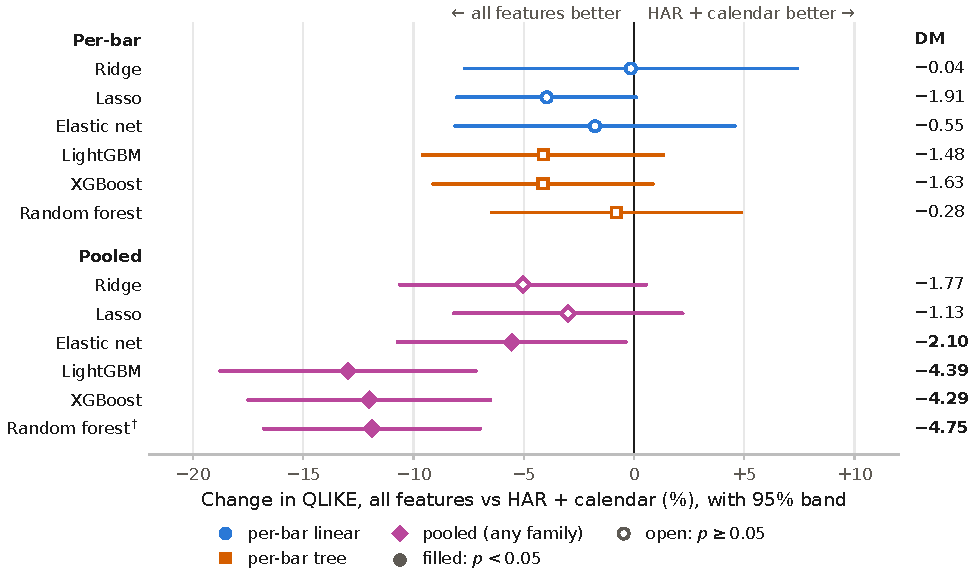
\includegraphics[width=\linewidth]{figures/rehaul_results_f1_forest.pdf}
% % 2026-10-15 (notation pass): parked -- code jargon (per-bar, family, HAR + calendar, all features, interim); standard terms and test wording
% % \caption{All features against HAR + calendar, within each family: the change in mean QLIKE (all features minus HAR +
% % calendar, in \% of the HAR + calendar value) with its 95\% band, $\Delta \pm 1.96\,|\Delta/\mathrm{DM}|$ (the interval
% % the Diebold--Mariano test inverts), and the DM statistic on the right (bold: $p < 0.05$). Left of zero, all features
% % forecast better. Colour and marker give the family for per-bar fits; every pooled fit is a diamond. Filled markers
% % have $p < 0.05$. $^\dagger$Interim (the pooled forest's 16:00 forecasts on all features). Numbers in
% % Table~\ref{tab:rh_axis1}.}
% \caption{Full predictor set versus HAR benchmark, by model class. For each model, the figure shows the change in
% mean QLIKE loss from the HAR benchmark to the full predictor set, in percent of the HAR-benchmark value, with its 95\%
% confidence interval $\Delta \pm 1.96\,|\Delta/\DM|$, obtained by inverting the Diebold--Mariano test; the $\DM$
% statistic is printed on the right. Negative values favor the full predictor set. Losses are computed against the
% actual realized variance of the closing half hour (15:30--16:00 ET) over the \rhrDays{} trading days of the
% out-of-sample period. Color and marker identify the model class of each closing-interval model; every pooled intraday
% model is drawn as a diamond. Filled markers and boldface: significant at the 5\% level (Diebold--Mariano test with
% the Harvey--Leybourne--Newbold correction, Newey--West lag $q = \fqsDMLag$). $^\dagger$Preliminary: the pooled
% random forest's closing-interval forecasts on the full predictor set. Table~\ref{tab:rh_axis1} reports the
% numbers.}
% \label{fig:rh_axis1_forest}
% \end{figure}

% ---------------------------------------------------------------- T2 + F2: pooled vs per-bar
% 2026-10-15 (user): parked -- "park all tables that I haven't mentioned in this chat"
% % AUTO-GENERATED by writeup/make_rehaul_results.py -- do not edit.
% tab:rh_axis2 (T2): intraday minus closing-interval, same model class and predictor set.
\begin{table}[htbp]
\centering
\small
\begin{threeparttable}
\caption{Forecast accuracy: closing-interval versus intraday models}
\label{tab:rh_axis2}
\begin{tabular}{@{}lrrrr@{}}
\toprule
 & \multicolumn{2}{c}{QLIKE} & \multicolumn{2}{c}{Sharpe ratio} \\
\cmidrule(lr){2-3}\cmidrule(l){4-5}
Model & $\Delta$ (\%) & $\DM$ & $\Delta\SR$ & $t$ \\
\midrule
\multicolumn{5}{@{}l}{\textit{Panel A: HAR benchmark}} \\
\addlinespace[2pt]
Ridge & $10.1^{***}$ & $(2.61)$ & $-0.49^{\phantom{***}}$ & $(-1.36)$ \\
Lasso & $10.1^{***}$ & $(2.61)$ & $-0.49^{\phantom{***}}$ & $(-1.36)$ \\
Elastic net & $10.1^{***}$ & $(2.61)$ & $-0.49^{\phantom{***}}$ & $(-1.36)$ \\
LightGBM & $0.7^{\phantom{***}}$ & $(0.23)$ & $0.29^{\phantom{***}}$ & $(0.26)$ \\
XGBoost & $2.4^{\phantom{***}}$ & $(0.84)$ & $0.15^{\phantom{***}}$ & $(0.67)$ \\
Random forest & $5.9^{*\phantom{**}}$ & $(1.86)$ & $-0.25^{\phantom{***}}$ & $(-0.46)$ \\
\addlinespace[4pt]
\multicolumn{5}{@{}l}{\textit{Panel B: Full predictor set}} \\
\addlinespace[2pt]
Ridge & $22.2^{***}$ & $(4.04)$ & $0.37^{\phantom{***}}$ & $(0.92)$ \\
Lasso & $31.2^{***}$ & $(4.64)$ & $0.28^{\phantom{***}}$ & $(0.12)$ \\
Elastic net & $21.6^{***}$ & $(4.16)$ & $0.26^{\phantom{***}}$ & $(0.07)$ \\
LightGBM & $3.9^{\phantom{***}}$ & $(1.18)$ & $0.56^{\phantom{***}}$ & $(0.60)$ \\
XGBoost & $4.6^{\phantom{***}}$ & $(1.34)$ & $0.58^{\phantom{***}}$ & $(0.68)$ \\
Random forest & $6.0^{*\phantom{**}}$ & $(1.84)$ & $1.11^{**\phantom{*}}$ & $(2.72)$ \\
\bottomrule
\end{tabular}
\begin{tablenotes}[flushleft]
\footnotesize
\item \textit{Notes:} Sample, loss and tests as in Table~\ref{tab:rh_axis1}. Each row compares the pooled intraday model with the closing-interval model of the same class on the predictor set of the panel: $\Delta = 100(\bar L^{\mathrm{pool}}/\bar L^{\mathrm{close}} - 1)$, positive when the closing-interval model is more accurate, and $\Delta\SR$ is the intraday minus the closing-interval Sharpe ratio. $^{*}$, $^{**}$ and $^{***}$ denote significance at the 10\%, 5\% and 1\% levels. Closing-interval trees use fixed hyperparameters and are re-estimated daily; the intraday trees are re-estimated at every interval, on a rolling window of past intervals (Section~\ref{sec:rh_exp_schemes}).
\end{tablenotes}
\end{threeparttable}
\end{table}


% 2026-10-15 (user): parked -- non-standard figure; focus on legible tables
% \begin{figure}[htbp]
% \centering
% 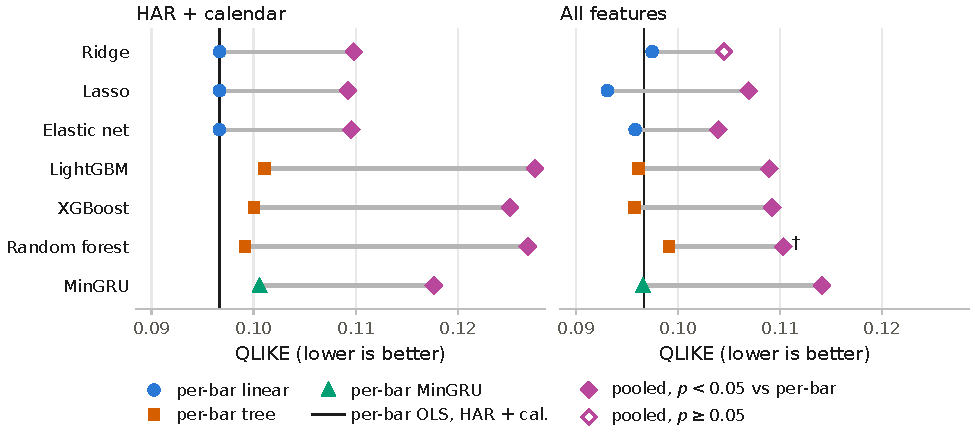
\includegraphics[width=\linewidth]{figures/rehaul_results_f2_dumbbell.pdf}
% % 2026-10-15 (notation pass): parked -- code jargon (per-bar, pooled fit, family, twin, session, interim); standard terms and test wording
% % \caption{Per-bar against pooled fits. Mean QLIKE of each family's per-bar fit (family colour and marker) and its
% % pooled fit (diamond), on HAR + calendar (left) and all features (right), on the same \rhrDays{} days; the vertical line
% % is the per-bar OLS on HAR + calendar (QLIKE \rhrOlsQ). A filled diamond is a pooled fit significantly worse than its
% % per-bar twin (Diebold--Mariano $p < 0.05$). Per-bar trees use fixed settings refit every session. $^\dagger$Interim.
% % Numbers in Table~\ref{tab:rh_axis2}.}
% \caption{Closing-interval versus pooled intraday models. The figure shows the mean QLIKE loss of each model class's
% closing-interval model (class color and marker) and of its pooled intraday counterpart (diamond), on the HAR benchmark
% (left) and on the full predictor set (right), over the same \rhrDays{} trading days of the out-of-sample period,
% against actual realized variance. The vertical line marks the closing-interval OLS on the HAR benchmark (mean QLIKE
% \rhrOlsQ). The closing-interval tree models use fixed hyperparameters and are re-estimated daily. Filled diamonds: the
% pooled intraday model is less accurate than its closing-interval counterpart, significant at the 5\% level
% (Diebold--Mariano test with the Harvey--Leybourne--Newbold correction, Newey--West lag $q = \fqsDMLag$).
% $^\dagger$Preliminary. Table~\ref{tab:rh_axis2} reports the numbers.}
% \label{fig:rh_pooled_dumbbell}
% \end{figure}

% ---------------------------------------------------------------- T3 + F3: the model set against the per-bar OLS
% 2026-10-15 (user): parked -- "park all tables that I haven't mentioned in this chat"
% % AUTO-GENERATED by writeup/make_rehaul_results.py -- do not edit.
\begin{table}[htbp]
\centering
\small
\setlength{\tabcolsep}{5pt}
\caption{The headline forecasts ranked by QLIKE, against the per-bar OLS on HAR + calendar. Rank is the position among all \rhrRankN{} forecasts of Table~\ref{tab:rh_rank_full}.}
\label{tab:rh_rank}
\begin{threeparttable}
\begin{tabular}{@{}r l l l r rrr@{}}
\toprule
 & & & & & \multicolumn{3}{c}{vs per-bar OLS} \\
\cmidrule(l){6-8}
Rank & Model & Fit & Inputs & QLIKE & $\Delta$ (\%) & DM & $p$ \\
\midrule
1 & Lasso & per-bar & All & 0.0914 & $-3.4$ & $-1.22$ & $0.222$ \\
2 & XGBoost, fixed, daily refit & per-bar & All & 0.0935 & $-1.2$ & $-0.39$ & $0.697$ \\
3 & LightGBM, fixed, daily refit & per-bar & All & 0.0939 & $-0.7$ & $-0.21$ & $0.831$ \\
4 & Elastic net & per-bar & All & 0.0942 & $-0.5$ & $-0.11$ & $0.915$ \\
8 & \textbf{OLS} (reference) & per-bar & HAR + cal. & \textbf{0.0946} & & & \\
9 & MinGRU (ridge-init, QLIKE-tuned) & per-bar & All & 0.0948 & $+0.2$ & $+0.05$ & $0.962$ \\
11 & Ridge & per-bar & All & 0.0958 & $+1.2$ & $+0.25$ & $0.799$ \\
14 & Random forest, fixed, daily refit & per-bar & All & 0.0966 & $+2.1$ & $+0.61$ & $0.543$ \\
16 & Random forest, fixed, daily refit & per-bar & HAR + cal. & 0.0968 & $+2.2$ & $+1.09$ & $0.276$ \\
21 & XGBoost, fixed, daily refit & per-bar & HAR + cal. & 0.0976 & $+3.1$ & $+1.43$ & $0.154$ \\
37 & MinGRU (ridge-init, QLIKE-tuned) & per-bar & HAR + cal. & 0.0985 & $+4.1$ & $+1.88$ & $0.060$ \\
38 & LightGBM, fixed, daily refit & per-bar & HAR + cal. & 0.0986 & $+4.2$ & $+1.92$ & $0.054$ \\
77 & Elastic net & pooled & All & 0.1016 & $+7.4$ & $+1.50$ & $0.134$ \\
81 & Ridge & pooled & All & 0.1021 & $+7.9$ & $+1.70$ & $0.090$ \\
93 & Lasso & pooled & All & 0.1044 & $+10.3$ & $\bm{+1.96}$ & $\bm{0.0497}$ \\
101 & LightGBM & pooled & All & 0.1060 & $+12.0$ & $\bm{+2.28}$ & $\bm{0.022}$ \\
102 & Lasso & pooled & HAR + cal. & 0.1062 & $+12.2$ & $\bm{+3.41}$ & $\bm{{<}0.001}$ \\
104 & XGBoost & pooled & All & 0.1063 & $+12.3$ & $\bm{+2.43}$ & $\bm{0.015}$ \\
105 & Elastic net & pooled & HAR + cal. & 0.1065 & $+12.6$ & $\bm{+3.49}$ & $\bm{{<}0.001}$ \\
107 & Ridge & pooled & HAR + cal. & 0.1067 & $+12.8$ & $\bm{+3.42}$ & $\bm{{<}0.001}$ \\
108 & Block-diagonal ridge, earlier panel & pooled & All & 0.1068 & $+12.8$ & $\bm{+2.38}$ & $\bm{0.017}$ \\
111 & Random forest$^\dagger$ & pooled & All & 0.1073 & $+13.4$ & $\bm{+2.53}$ & $\bm{0.011}$ \\
115 & MinGRU (ridge-init, QLIKE-tuned) & pooled & All & 0.1121 & $+18.4$ & $\bm{+4.53}$ & $\bm{{<}0.001}$ \\
116 & MinGRU (ridge-init, QLIKE-tuned) & pooled & HAR + cal. & 0.1151 & $+21.7$ & $\bm{+4.88}$ & $\bm{{<}0.001}$ \\
117 & XGBoost & pooled & HAR + cal. & 0.1213 & $+28.2$ & $\bm{+5.03}$ & $\bm{{<}0.001}$ \\
118 & Random forest & pooled & HAR + cal. & 0.1229 & $+29.9$ & $\bm{+5.04}$ & $\bm{{<}0.001}$ \\
119 & OLS, earlier panel & pooled & HAR + cal. & 0.1232 & $+30.2$ & $\bm{+4.80}$ & $\bm{{<}0.001}$ \\
120 & LightGBM & pooled & HAR + cal. & 0.1236 & $+30.7$ & $\bm{+5.02}$ & $\bm{{<}0.001}$ \\
\bottomrule
\end{tabular}
\begin{tablenotes}[flushleft]\footnotesize
\item \textit{Notes.} QLIKE is the mean over the \rhrDays{} trade days (2020-01-03 to 2024-04-30, early closes excluded) of the daily loss $L_t = RV_t/\hat\sigma^2_t - \log(RV_t/\hat\sigma^2_t) - 1$, with the plain forecast $\hat\sigma^2_t = \hat y_t^2 B_t$ (no recalibration) and $RV_t$ the winsorised 15:30--16:00 realised variance. $\Delta = 100(\overline{L}/\overline{L}^{\,\text{OLS}} - 1)$. DM is the Diebold--Mariano statistic of the daily QLIKE difference (model minus the per-bar OLS), with a Bartlett Newey--West variance at lag 6 and the Harvey--Leybourne--Newbold correction; $p$ is two-sided (normal). Negative $\Delta$ and DM favour the model. Bold: $p < 0.05$. Rows: the per-bar OLS, the canonical rung of each family on each input set (per-bar trees with fixed settings refit every session) and the earlier paper's pooled OLS and block-diagonal ridge. The per-bar ridge, lasso and elastic net on HAR + calendar are within \rhrLinBaseMaxPct\,\% of the OLS and are not shown. $^\dagger$Interim (see Table~\ref{tab:rh_axis1}). The pooled MinGRU is refit monthly, the pooled trees at every bar. Of the \rhrNSet{} model-set forecasts other than the OLS, \rhrNLower{} have lower QLIKE (\rhrNLowerSig{} with $p < 0.05$) and \rhrNWorseSig{} are significantly worse.
\end{tablenotes}
\end{threeparttable}
\end{table}


% 2026-10-15 (user): parked -- "I need all plots parked"
% \begin{figure}[htbp]
% \centering
% 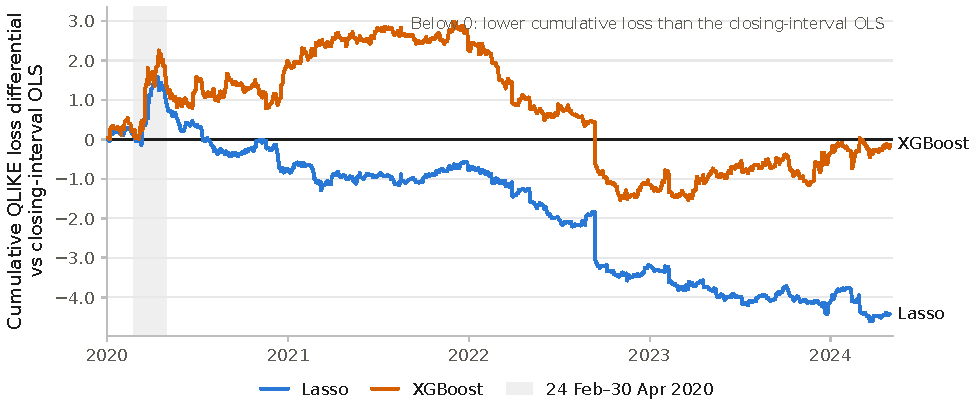
\includegraphics[width=\linewidth]{figures/rehaul_results_f3_cumulative.pdf}
% % 2026-10-15 (notation pass): parked -- code jargon (per-bar, family, fixed settings, session); dummy day index s -> u (s is the window row)
% % \caption{Cumulative daily QLIKE difference against the per-bar OLS on HAR + calendar, $\sum_{s \le t}
% % (L_s^{\text{model}} - L_s^{\text{OLS}})$, for the best per-bar forecast of each family, all on all features: the lasso,
% % XGBoost (fixed settings, refit every session) and the MinGRU (ridge-initialised, trained and selected on QLIKE). Below
% % zero, the model has accumulated less QLIKE than the OLS; the end value divided by \rhrDays{} is the difference in mean
% % QLIKE. Over the shaded window, 24 February to 30 April 2020, the sums change by \rhrCumLassoWindow{} (lasso),
% % \rhrCumXgbWindow{} (XGBoost) and \rhrCumNnWindow{} (MinGRU); over the full sample they end at \rhrCumLassoTotal,
% % \rhrCumXgbTotal{} and \rhrCumNnTotal.}
% % 2026-10-15 (consolidation): dummy day index u -> t' (u is an exogenous series); cumulative-loss plot in the style
% % of \citet{WelchGoyal2008}, now cited.
% % 2026-10-15 (user): parked -- NN content parked for now. The caption below drops the MinGRU line, its
% % \rhrCumNnWindow / \rhrCumNnTotal macros and "the network (ridge-initialized, trained and selected on QLIKE)"; the
% % generator agent drops the MinGRU line from the figure. Old caption: "... the lasso, XGBoost (fixed hyperparameters,
% % re-estimated daily) and the MinGRU network (ridge-initialized, trained and selected on QLIKE) ... change by
% % \rhrCumLassoWindow{} (lasso), \rhrCumXgbWindow{} (XGBoost) and \rhrCumNnWindow{} (MinGRU); over the full
% % out-of-sample period they end at \rhrCumLassoTotal, \rhrCumXgbTotal{} and \rhrCumNnTotal."
% \caption{Cumulative QLIKE loss differential relative to the closing-interval OLS on the HAR benchmark. The figure
% plots $\sum_{t' \le t} d_{t'}$, where $d_{t'} = L_{t'}^{\text{model}} - L_{t'}^{\text{OLS}}$ is the daily loss
% differential, as in \citet{WelchGoyal2008}, for the closing-interval model with the lowest mean QLIKE in each model
% class, each on the full predictor set: the lasso and XGBoost (fixed hyperparameters, re-estimated daily). Values below
% zero mean that the model has accumulated a smaller loss than the OLS; the final value divided by \rhrDays{} equals the
% difference in mean QLIKE. Losses are computed against actual realized variance. Over the shaded window, 24 February to
% 30 April 2020, the cumulative differentials change by \rhrCumLassoWindow{} (lasso) and \rhrCumXgbWindow{} (XGBoost);
% over the full out-of-sample period they end at \rhrCumLassoTotal{} and \rhrCumXgbTotal.}
% \label{fig:rh_cumulative}
% \end{figure}

% ---------------------------------------------------------------- F5: why QLIKE is the primary loss
% 2026-10-15 (user): parked -- non-standard figure; focus on legible tables
% \begin{figure}[htbp]
% \centering
% 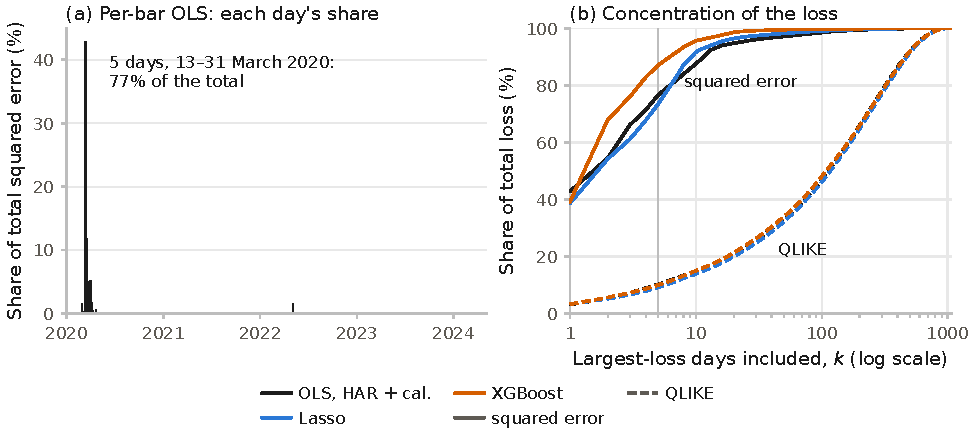
\includegraphics[width=\linewidth]{figures/rehaul_results_f5_se_share.pdf}
% % 2026-10-15 (notation pass): parked -- RV_t -> \RV_t; per-bar, input-set pairs, all features; significance wording
% % \caption{Concentration of the loss. (a) Each day's share of the per-bar OLS's total squared error,
% % $\sum_t (RV_t - \hat\sigma^2_t)^2$: its five largest days, all in March 2020, carry \rhrSETopFiveOls\% of it.
% % (b) Share of the total loss carried by the $k$ largest-loss days, for squared error (solid) and QLIKE (dashed), for the
% % OLS and the three forecasts of Figure~\ref{fig:rh_cumulative}. For each of the four, the five largest squared errors
% % fall in March 2020 and carry \rhrSETopFiveMin--\rhrSETopFiveMax\% of the total squared error; the five largest QLIKE
% % days carry \rhrQLTopFiveMin--\rhrQLTopFiveMax\% of the total QLIKE. Across the \rhrAfPairs{} input-set pairs, all
% % features raise the squared error in \rhrAfMseHigher{} (\rhrAfMseHigherSig{} significantly) while lowering QLIKE in
% % \rhrAfLower.}
% \caption{Concentration of squared-error and QLIKE losses. Panel (a): each trading day's share of the total
% squared-error loss of the closing-interval OLS on the HAR benchmark, $\sum_t (\RV_t - \hat\sigma^2_t)^2$; its five
% largest days, all in March 2020, account for \rhrSETopFiveOls\% of the total. Panel (b): share of the total loss
% accounted for by the $k$ largest-loss days, under squared-error loss (solid) and QLIKE (dashed), for the OLS and the
% three forecasts of Figure~\ref{fig:rh_cumulative}. For each of the four, the five largest squared errors fall in March
% 2020 and account for \rhrSETopFiveMin--\rhrSETopFiveMax\% of the total squared-error loss; the five largest QLIKE
% losses account for \rhrQLTopFiveMin--\rhrQLTopFiveMax\% of the total QLIKE. Across the \rhrAfPairs{} specifications
% estimated on both predictor sets, the full predictor set raises the squared-error loss in \rhrAfMseHigher{}
% (\rhrAfMseHigherSig{} significant at the 5\% level) and lowers QLIKE in \rhrAfLower. Losses are computed against actual
% realized variance over the \rhrDays{} trading days of the out-of-sample period; significance by the Diebold--Mariano
% test with the Harvey--Leybourne--Newbold correction (Newey--West lag $q = \fqsDMLag$).}
% \label{fig:rh_se_share}
% \end{figure}

% ---------------------------------------------------------------- existing figure: QLIKE vs Sharpe (economics bridge)
% figures/fig_qlike_sharpe.pdf and its \fqs... macros come from writeup/make_fig_qlike_sharpe.py (its own palette: one
% colour per estimator, not the family colours above).
% 2026-10-15 parked: the same figure is placed in 07_economics_floats.tex (fig:rh_econ_qlike_sharpe); one copy kept.
% \begin{figure}[htbp]
% \centering
% 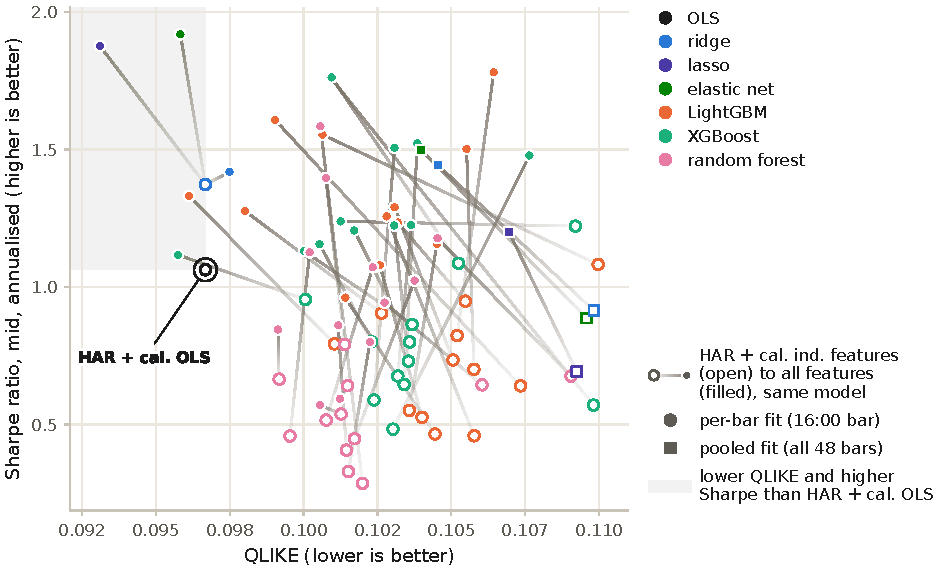
\includegraphics[width=\linewidth]{figures/fig_qlike_sharpe.pdf}
% \caption{Mean QLIKE against the Sharpe ratio of the midpoint straddle trade for every model of the set fitted on both
% input sets: \fqsPairs{} pairs (\fqsPairsPerBarLinear{} per-bar linear, \fqsPairsPooled{} pooled linear and
% \fqsPairsTree{} per-bar trees), on the same \fqsDays{} days. Each pair is joined from its HAR + calendar end (open
% marker) to its all-features end (filled marker); circles are per-bar fits, squares pooled fits, and the colour marks
% the estimator. The shaded quadrant holds lower QLIKE and a higher Sharpe ratio than the per-bar OLS on HAR + calendar
% (QLIKE \fqsOlsQ, Sharpe \fqsOlsSh). All features raise the Sharpe ratio in \fqsShHigher{} of the \fqsPairs{} pairs
% (\fqsShHigherSig{} significant by the Newey--West $t$ of the daily return difference, lag \fqsHACLag) and lower QLIKE
% in \fqsQLower{} (\fqsQLowerSig{} significant by Diebold--Mariano, lag \fqsDMLag); significance at \fqsSigPct\%.}
% \label{fig:rh_qlike_sharpe}
% \end{figure}

% ---------------------------------------------------------------- T3 (full): every forecast, a longtable
% Not a float: \clearpage first so T1--T3 and the figures above come out before it. A candidate for the appendix.
% 2026-10-15 (consolidation): parked -- moved to the appendix (10_appendix_floats.tex, after the MinGRU tables).
% \clearpage
% % AUTO-GENERATED by writeup/make_rehaul_results.py -- do not edit.
% tab:rh_rank_full (T3, every forecast): a longtable, for the appendix (10_appendix_floats.tex).
{\small
\setlength{\tabcolsep}{3.5pt}
\begin{longtable}{@{}rlllrrr@{}}
\caption{Ranking of all forecasts by mean QLIKE}
\label{tab:rh_rank_full}\\
\toprule
 & & & & & \multicolumn{2}{c}{vs.\ HAR benchmark} \\
\cmidrule(l){6-7}
Rank & Model & Specification & Predictors & QLIKE & $\Delta$ (\%) & $\DM$ \\
\midrule
\endfirsthead
\multicolumn{7}{@{}l}{\textit{Table~\ref{tab:rh_rank_full}, continued}} \\
\toprule
 & & & & & \multicolumn{2}{c}{vs.\ HAR benchmark} \\
\cmidrule(l){6-7}
Rank & Model & Specification & Predictors & QLIKE & $\Delta$ (\%) & $\DM$ \\
\midrule
\endhead
\midrule
\multicolumn{7}{r@{}}{\textit{Continued on next page}} \\
\endfoot
\bottomrule
\multicolumn{7}{@{}p{\linewidth}@{}}{\footnotesize\raggedright \textit{Notes:} Sample, loss, tests and significance markers as in Table~\ref{tab:rh_axis1}; $\Delta$ and $\DM$ compare each forecast with the HAR benchmark, as in Table~\ref{tab:rh_rank}. Specification of the closing-interval trees (Panel A): fixed hyperparameters, random search or Optuna, selecting on MSE or QLIKE, then the re-estimation frequency or, for Optuna, the re-tuning frequency and the number of trials searched; d: trading days (Section~\ref{sec:rh_methods_tuning}). Panel C holds the earlier draft's intraday linear models, with a block, fixed or re-tuned penalty; ``no FOMC'' marks the earlier draft's predictor set, which lacks the FOMC predictors. The intraday models of Panel B are re-estimated at every interval on the \rhePoolNBars{} regular-hours intervals with a rolling window of \rhePoolWindowDays{} trading days (Section~\ref{sec:rh_exp_schemes}), except the linear models marked ``All \rhdmNIntervals{} intervals'', the runs on every interval of the day in the model set. $^{\ddagger}$Not in the model set counted in the text.} \tabularnewline
\endlastfoot
\multicolumn{7}{@{}l}{\textit{Panel A: Closing-interval models}} \\
\addlinespace[2pt]
1 & Lasso & -- & Full & 0.0992 & $-4.0^{*\phantom{**}}$ & $(-1.91)$ \\
2 & Elastic net & -- & Full & 0.1014 & $-1.8^{\phantom{***}}$ & $(-0.55)$ \\
3 & Ridge & -- & Full & 0.1031 & $-0.1^{\phantom{***}}$ & $(-0.04)$ \\
4 & XGBoost & Fixed, daily & Full & 0.1031 & $-0.1^{\phantom{***}}$ & $(-0.04)$ \\
5 & Lasso & -- & HAR & 0.1033 & $0.0^{***}$ & $(-2.60)$ \\
6 & Elastic net & -- & HAR & 0.1033 & $0.0^{**\phantom{*}}$ & $(-2.46)$ \\
7 & Ridge & -- & HAR & 0.1033 & $0.0^{\phantom{***}}$ & $(-0.96)$ \\
8 & OLS (benchmark) & -- & HAR & 0.1033 & --$^{\phantom{***}}$ & -- \\
9 & LightGBM & Fixed, daily & Full & 0.1049 & $1.5^{\phantom{***}}$ & $(0.51)$ \\
10 & Random forest & Random search (QLIKE), every 10 d & HAR & 0.1058 & $2.4^{\phantom{***}}$ & $(1.18)$ \\
11 & Random forest & Fixed, daily & Full & 0.1060 & $2.6^{\phantom{***}}$ & $(0.86)$ \\
12 & LightGBM & Fixed, every 10 d & Full & 0.1061 & $2.7^{\phantom{***}}$ & $(0.86)$ \\
13 & Random forest & Optuna (QLIKE), 25 d, 50 trials & HAR & 0.1062 & $2.8^{\phantom{***}}$ & $(1.36)$ \\
14 & LightGBM & Random search (QLIKE), daily & Full & 0.1063 & $3.0^{\phantom{***}}$ & $(0.94)$ \\
15 & Random forest & Random search (QLIKE), daily & HAR & 0.1065 & $3.1^{\phantom{***}}$ & $(1.56)$ \\
16 & XGBoost & Fixed, every 10 d & Full & 0.1066 & $3.2^{\phantom{***}}$ & $(0.89)$ \\
17 & LightGBM & Random search (MSE), daily & Full & 0.1068 & $3.5^{\phantom{***}}$ & $(0.97)$ \\
18 & Random forest & Fixed, daily & HAR & 0.1068 & $3.5^{*\phantom{**}}$ & $(1.70)$ \\
19 & Random forest & Optuna (MSE), daily, 10 trials & Full & 0.1070 & $3.6^{\phantom{***}}$ & $(1.12)$ \\
20 & Random forest & Optuna (MSE), daily, 25 trials & Full & 0.1070 & $3.6^{\phantom{***}}$ & $(1.16)$ \\
21 & Random forest & Optuna (MSE), 5 d, 50 trials & Full & 0.1071 & $3.7^{\phantom{***}}$ & $(1.08)$ \\
22 & XGBoost & Fixed, every 10 d & HAR & 0.1072 & $3.8^{*\phantom{**}}$ & $(1.83)$ \\
23 & Random forest & Optuna (MSE), daily, 50 trials & Full & 0.1072 & $3.8^{\phantom{***}}$ & $(1.18)$ \\
24 & Random forest & Random search (QLIKE), daily & Full & 0.1073 & $3.9^{\phantom{***}}$ & $(1.29)$ \\
25 & XGBoost & Optuna (MSE), daily, 25 trials & Full & 0.1073 & $3.9^{\phantom{***}}$ & $(1.13)$ \\
26 & Random forest & Optuna (MSE), 25 d, 10 trials & Full & 0.1073 & $3.9^{\phantom{***}}$ & $(1.21)$ \\
27 & Random forest & Optuna (MSE), daily, 50 trials & HAR & 0.1074 & $4.0^{*\phantom{**}}$ & $(1.79)$ \\
28 & Random forest & Optuna (MSE), daily, 25 trials & HAR & 0.1075 & $4.1^{*\phantom{**}}$ & $(1.94)$ \\
29 & XGBoost & Fixed, daily & HAR & 0.1076 & $4.2^{**\phantom{*}}$ & $(2.09)$ \\
30 & Random forest & Fixed, every 10 d & Full & 0.1076 & $4.2^{\phantom{***}}$ & $(1.30)$ \\
31 & LightGBM & Random search (QLIKE), every 10 d & Full & 0.1076 & $4.2^{\phantom{***}}$ & $(1.16)$ \\
32 & Random forest & Optuna (MSE), 25 d, 25 trials & HAR & 0.1077 & $4.3^{*\phantom{**}}$ & $(1.82)$ \\
33 & Random forest & Optuna (MSE), 5 d, 50 trials & HAR & 0.1078 & $4.4^{*\phantom{**}}$ & $(1.89)$ \\
34 & XGBoost & Random search (MSE), daily & Full & 0.1078 & $4.4^{\phantom{***}}$ & $(1.17)$ \\
35 & XGBoost & Random search (QLIKE), daily & Full & 0.1078 & $4.4^{\phantom{***}}$ & $(1.18)$ \\
36 & Random forest & Optuna (MSE), daily, 10 trials & HAR & 0.1078 & $4.4^{**\phantom{*}}$ & $(2.09)$ \\
38 & LightGBM & Random search (MSE), every 10 d & Full & 0.1079 & $4.4^{\phantom{***}}$ & $(1.14)$ \\
40 & Random forest & Optuna (MSE), 25 d, 50 trials & HAR & 0.1080 & $4.6^{**\phantom{*}}$ & $(1.98)$ \\
41 & Random forest & Fixed, every 10 d & HAR & 0.1081 & $4.6^{**\phantom{*}}$ & $(2.15)$ \\
42 & Random forest & Optuna (MSE), 25 d, 25 trials & Full & 0.1082 & $4.7^{\phantom{***}}$ & $(1.49)$ \\
43 & XGBoost & Optuna (MSE), 5 d, 50 trials & HAR & 0.1082 & $4.8^{**\phantom{*}}$ & $(2.15)$ \\
44 & XGBoost & Optuna (MSE), daily, 10 trials & HAR & 0.1085 & $5.1^{**\phantom{*}}$ & $(2.14)$ \\
46 & LightGBM & Optuna (MSE), 250 d, 50 trials & Full & 0.1086 & $5.2^{\phantom{***}}$ & $(1.26)$ \\
47 & Random forest & Optuna (MSE), 25 d, 10 trials & HAR & 0.1088 & $5.3^{**\phantom{*}}$ & $(2.03)$ \\
48 & XGBoost & Optuna (MSE), daily, 50 trials & Full & 0.1089 & $5.5^{*\phantom{**}}$ & $(1.67)$ \\
50 & Random forest & Optuna (MSE), 250 d, 50 trials & Full & 0.1090 & $5.5^{*\phantom{**}}$ & $(1.66)$ \\
51 & Random forest & Optuna (QLIKE), 25 d, 50 trials & Full & 0.1091 & $5.7^{\phantom{***}}$ & $(1.63)$ \\
52 & XGBoost & Optuna (MSE), 25 d, 50 trials & HAR & 0.1091 & $5.7^{**\phantom{*}}$ & $(2.21)$ \\
53 & LightGBM & Fixed, daily & HAR & 0.1094 & $5.9^{***}$ & $(2.70)$ \\
54 & XGBoost & Optuna (MSE), 5 d, 50 trials & Full & 0.1094 & $6.0^{*\phantom{**}}$ & $(1.77)$ \\
55 & LightGBM & Optuna (MSE), daily, 10 trials & Full & 0.1095 & $6.0^{*\phantom{**}}$ & $(1.65)$ \\
56 & LightGBM & Random search (QLIKE), every 10 d & HAR & 0.1095 & $6.1^{***}$ & $(2.79)$ \\
57 & LightGBM & Optuna (MSE), daily, 25 trials & Full & 0.1096 & $6.1^{*\phantom{**}}$ & $(1.75)$ \\
58 & LightGBM & Random search (QLIKE), daily & HAR & 0.1097 & $6.2^{***}$ & $(2.85)$ \\
59 & XGBoost & Random search (QLIKE), every 10 d & Full & 0.1098 & $6.3^{\phantom{***}}$ & $(1.53)$ \\
60 & XGBoost & Random search (MSE), every 10 d & Full & 0.1098 & $6.3^{\phantom{***}}$ & $(1.55)$ \\
61 & LightGBM & Fixed, every 10 d & HAR & 0.1098 & $6.4^{***}$ & $(2.80)$ \\
62 & XGBoost & Optuna (MSE), daily, 50 trials & HAR & 0.1099 & $6.4^{**\phantom{*}}$ & $(2.57)$ \\
63 & Random forest & Random search (QLIKE), every 10 d & Full & 0.1099 & $6.4^{*\phantom{**}}$ & $(1.91)$ \\
64 & Random forest & Optuna (MSE), 25 d, 50 trials & Full & 0.1100 & $6.5^{*\phantom{**}}$ & $(1.89)$ \\
65 & LightGBM & Optuna (MSE), 25 d, 25 trials & HAR & 0.1100 & $6.5^{***}$ & $(2.81)$ \\
66 & XGBoost & Optuna (QLIKE), 25 d, 50 trials & HAR & 0.1101 & $6.6^{*\phantom{**}}$ & $(1.93)$ \\
70 & XGBoost & Optuna (MSE), daily, 25 trials & HAR & 0.1102 & $6.7^{**\phantom{*}}$ & $(2.56)$ \\
71 & XGBoost & Optuna (MSE), 25 d, 10 trials & HAR & 0.1102 & $6.7^{***}$ & $(2.93)$ \\
72 & LightGBM & Optuna (MSE), daily, 50 trials & Full & 0.1103 & $6.8^{**\phantom{*}}$ & $(1.97)$ \\
73 & XGBoost & Optuna (MSE), 25 d, 25 trials & HAR & 0.1103 & $6.8^{**\phantom{*}}$ & $(2.53)$ \\
74 & LightGBM & Optuna (QLIKE), 25 d, 50 trials & HAR & 0.1104 & $6.9^{***}$ & $(2.87)$ \\
75 & LightGBM & Optuna (MSE), 5 d, 50 trials & Full & 0.1104 & $6.9^{*\phantom{**}}$ & $(1.87)$ \\
76 & XGBoost & Optuna (MSE), daily, 10 trials & Full & 0.1106 & $7.1^{**\phantom{*}}$ & $(2.00)$ \\
77 & LightGBM & Optuna (MSE), daily, 10 trials & HAR & 0.1110 & $7.5^{***}$ & $(2.78)$ \\
78 & XGBoost & Optuna (MSE), 250 d, 50 trials & Full & 0.1111 & $7.6^{*\phantom{**}}$ & $(1.69)$ \\
79 & LightGBM & Optuna (MSE), 25 d, 25 trials & Full & 0.1112 & $7.6^{*\phantom{**}}$ & $(1.87)$ \\
80 & LightGBM & Optuna (MSE), 25 d, 50 trials & HAR & 0.1112 & $7.7^{***}$ & $(2.82)$ \\
81 & LightGBM & Optuna (MSE), 5 d, 50 trials & HAR & 0.1114 & $7.9^{***}$ & $(3.27)$ \\
83 & Random forest & Random search (MSE), daily & Full & 0.1117 & $8.1^{**\phantom{*}}$ & $(1.98)$ \\
84 & LightGBM & Optuna (MSE), daily, 50 trials & HAR & 0.1117 & $8.1^{***}$ & $(3.01)$ \\
85 & Random forest & Optuna (MSE), 250 d, 50 trials & HAR & 0.1121 & $8.6^{**\phantom{*}}$ & $(2.00)$ \\
86 & LightGBM & Optuna (MSE), 25 d, 10 trials & HAR & 0.1122 & $8.7^{***}$ & $(3.29)$ \\
89 & XGBoost & Optuna (MSE), 25 d, 25 trials & Full & 0.1126 & $9.0^{**\phantom{*}}$ & $(2.26)$ \\
91 & XGBoost & Random search (QLIKE), daily & HAR & 0.1127 & $9.1^{**\phantom{*}}$ & $(1.96)$ \\
92 & LightGBM & Optuna (MSE), daily, 25 trials & HAR & 0.1127 & $9.2^{***}$ & $(3.26)$ \\
93 & XGBoost & Random search (QLIKE), every 10 d & HAR & 0.1127 & $9.2^{*\phantom{**}}$ & $(1.93)$ \\
95 & LightGBM & Optuna (MSE), 25 d, 10 trials & Full & 0.1128 & $9.3^{**\phantom{*}}$ & $(2.03)$ \\
97 & XGBoost & Optuna (QLIKE), 25 d, 50 trials & Full & 0.1134 & $9.8^{**\phantom{*}}$ & $(2.25)$ \\
98 & LightGBM & Optuna (QLIKE), 25 d, 50 trials & Full & 0.1134 & $9.9^{**\phantom{*}}$ & $(2.10)$ \\
100 & XGBoost & Optuna (MSE), 25 d, 50 trials & Full & 0.1136 & $10.0^{**\phantom{*}}$ & $(2.42)$ \\
101 & LightGBM & Random search (MSE), every 10 d & HAR & 0.1136 & $10.0^{**\phantom{*}}$ & $(2.51)$ \\
105 & LightGBM & Random search (MSE), daily & HAR & 0.1139 & $10.3^{***}$ & $(2.59)$ \\
110 & Random forest & Random search (MSE), every 10 d & HAR & 0.1149 & $11.3^{**\phantom{*}}$ & $(2.33)$ \\
111 & Random forest & Random search (MSE), daily & HAR & 0.1151 & $11.5^{**\phantom{*}}$ & $(2.40)$ \\
112 & LightGBM & Optuna (MSE), 25 d, 50 trials & Full & 0.1152 & $11.6^{***}$ & $(2.61)$ \\
113 & Random forest & Random search (MSE), every 10 d & Full & 0.1157 & $12.1^{**\phantom{*}}$ & $(2.20)$ \\
115 & LightGBM & Optuna (MSE), 250 d, 50 trials & HAR & 0.1160 & $12.3^{***}$ & $(2.84)$ \\
116 & XGBoost & Optuna (MSE), 25 d, 10 trials & Full & 0.1161 & $12.4^{***}$ & $(2.72)$ \\
117 & XGBoost & Optuna (MSE), 250 d, 50 trials & HAR & 0.1165 & $12.8^{***}$ & $(3.24)$ \\
119 & XGBoost & Random search (MSE), every 10 d & HAR & 0.1174 & $13.7^{***}$ & $(2.77)$ \\
120 & XGBoost & Random search (MSE), daily & HAR & 0.1175 & $13.8^{***}$ & $(2.78)$ \\
\addlinespace[4pt]
\multicolumn{7}{@{}l}{\textit{Panel B: Intraday models}} \\
\addlinespace[2pt]
37 & Elastic net & All \rhdmNIntervals{} intervals & Full & 0.1078 & $4.4^{\phantom{***}}$ & $(1.17)$ \\
39 & XGBoost$^{\ddagger}$ & -- & Full & 0.1079 & $4.5^{\phantom{***}}$ & $(1.14)$ \\
45 & Ridge & All \rhdmNIntervals{} intervals & Full & 0.1086 & $5.1^{\phantom{***}}$ & $(1.36)$ \\
49 & LightGBM$^{\ddagger}$ & -- & Full & 0.1089 & $5.5^{\phantom{***}}$ & $(1.34)$ \\
67 & LightGBM$^{\ddagger}$ & -- & HAR & 0.1101 & $6.6^{**\phantom{*}}$ & $(2.16)$ \\
68 & Lasso & All \rhdmNIntervals{} intervals & Full & 0.1101 & $6.7^{\phantom{***}}$ & $(1.62)$ \\
69 & XGBoost$^{\ddagger}$ & -- & HAR & 0.1102 & $6.7^{**\phantom{*}}$ & $(2.23)$ \\
88 & Random forest$^{\ddagger}$ & -- & Full & 0.1123 & $8.8^{**\phantom{*}}$ & $(2.06)$ \\
90 & XGBoost & Earlier draft, no FOMC & Full & 0.1126 & $9.0^{**\phantom{*}}$ & $(2.18)$ \\
94 & LightGBM & Earlier draft, no FOMC & Full & 0.1128 & $9.2^{**\phantom{*}}$ & $(2.16)$ \\
96 & Random forest$^{\ddagger}$ & -- & HAR & 0.1131 & $9.6^{***}$ & $(2.78)$ \\
99 & Lasso & All \rhdmNIntervals{} intervals & HAR & 0.1135 & $10.0^{***}$ & $(3.09)$ \\
102 & Elastic net$^{\ddagger}$ & -- & HAR & 0.1137 & $10.1^{***}$ & $(2.61)$ \\
103 & Lasso$^{\ddagger}$ & -- & HAR & 0.1137 & $10.1^{***}$ & $(2.61)$ \\
104 & Ridge$^{\ddagger}$ & -- & HAR & 0.1137 & $10.1^{***}$ & $(2.61)$ \\
107 & Elastic net & All \rhdmNIntervals{} intervals & HAR & 0.1142 & $10.6^{***}$ & $(3.21)$ \\
109 & Ridge & All \rhdmNIntervals{} intervals & HAR & 0.1143 & $10.7^{***}$ & $(3.15)$ \\
121 & Elastic net$^{\ddagger}$ & -- & Full & 0.1234 & $19.5^{***}$ & $(3.34)$ \\
122 & Ridge$^{\ddagger}$ & -- & Full & 0.1260 & $22.0^{***}$ & $(3.61)$ \\
124 & Lasso$^{\ddagger}$ & -- & Full & 0.1301 & $26.0^{***}$ & $(3.66)$ \\
\addlinespace[4pt]
\multicolumn{7}{@{}l}{\textit{Panel C: Intraday models, earlier draft's specification}} \\
\addlinespace[2pt]
82 & Lasso & Fixed penalty, no FOMC & Full & 0.1116 & $8.1^{*\phantom{**}}$ & $(1.87)$ \\
87 & Ridge & Block penalty, no FOMC & Full & 0.1123 & $8.8^{**\phantom{*}}$ & $(1.96)$ \\
106 & Ridge & Block penalty & Full & 0.1140 & $10.4^{**\phantom{*}}$ & $(2.27)$ \\
108 & Lasso & Fixed penalty & Full & 0.1143 & $10.7^{**\phantom{*}}$ & $(2.37)$ \\
114 & Lasso & Re-tuned penalty, no FOMC & Full & 0.1158 & $12.1^{***}$ & $(2.64)$ \\
118 & Elastic net & Re-tuned penalty, no FOMC & Full & 0.1174 & $13.6^{***}$ & $(2.95)$ \\
123 & OLS & -- & HAR & 0.1291 & $25.0^{***}$ & $(4.56)$ \\
\end{longtable}
}

